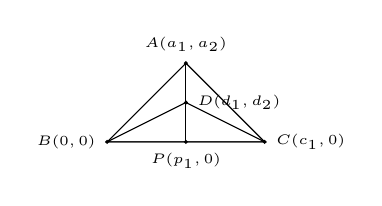
\begin{tikzpicture}
%[scale=0.5,>=stealth,point/.style={draw,circle,fill = green,inner sep=0.1pt},]
[scale=0.5,>=stealth, point/.style={draw,circle,fill = black,inner sep=0.1pt}]

% the coordinates of the vertices
\coordinate (A) at (2,2);
\coordinate (B) at (0,0);
\coordinate (C) at (4,0);
\coordinate (D) at (2,1);
\coordinate (P) at (2,0);


% the axis
\draw[thin,scale=0,-] (-1,0) -- (5.5,0);
\draw[thin,scale=0,-] (0,-2.5) -- (0,2.5);
\draw[thin,scale=0,-] (0,-2.5) -- (0,2.5);

% the edges of the triangle
\draw (B) -- (A) -- (C)-- cycle;
\draw (B) -- (D) -- (C)-- cycle;
\draw[-] (A) -- (D) ;
\draw[-] (P) -- (D) ;


% labelling the vertices
\node[point,label={above:\tiny $A (a_1,a_2)$}] at (A) {};
\node[point,label={left:\tiny $B(0,0)$}] at (B) {};
\node[point,label={right:\tiny $C(c_1,0)$}] at (C) {};
\node[point,label={right:\tiny $D(d_1,d_2)$}] at (D) {};
\node[point,label={below:\tiny $P(p_1,0)$}] at (P) {};



%
\end{tikzpicture}
